\documentclass[10pt]{article}
\usepackage[margin=0.5in]{geometry}
\usepackage[T1]{fontenc}
\usepackage{tikz}
\usepackage{pgfplots}
\usepackage{subcaption}
\usepackage[table]{xcolor}
\usetikzlibrary{arrows.meta,positioning,calc,fit,backgrounds,shapes.geometric}
\pgfplotsset{compat=1.18}
\pagestyle{empty}

\definecolor{navy}{HTML}{16324F}
\definecolor{teal}{HTML}{2F6F6D}
\definecolor{gold}{HTML}{C78A2C}
\definecolor{brick}{HTML}{B24745}
\definecolor{slate}{HTML}{6B7A8F}
\definecolor{softgray}{HTML}{F3F5F7}
\definecolor{blanket}{HTML}{DCEFE7}

\tikzset{
  flowbox/.style={
    rounded corners=7pt,
    draw=navy!70,
    fill=softgray,
    thick,
    minimum width=2.1cm,
    minimum height=0.95cm,
    align=center,
    font=\footnotesize
  },
  modelbox/.style={
    rounded corners=7pt,
    draw=teal!75!black,
    fill=teal!8,
    thick,
    minimum width=2.2cm,
    minimum height=1.0cm,
    align=center,
    font=\footnotesize
  },
  evalbox/.style={
    rounded corners=7pt,
    draw=gold!85!black,
    fill=gold!12,
    thick,
    minimum width=2.2cm,
    minimum height=1.0cm,
    align=center,
    font=\footnotesize
  },
  dataarrow/.style={-{Latex[length=2.6mm,width=1.8mm]},thick,draw=navy!75},
  dagroot/.style={ellipse,draw=navy!70,fill=navy!10,thick,minimum width=1.05cm,minimum height=0.55cm,font=\scriptsize},
  dagnode/.style={ellipse,draw=teal!75!black,fill=teal!10,thick,minimum width=1.1cm,minimum height=0.55cm,font=\scriptsize},
  dagparent/.style={ellipse,draw=gold!80!black,fill=gold!18,thick,minimum width=1.1cm,minimum height=0.55cm,font=\scriptsize},
  dagtarget/.style={ellipse,draw=brick!80!black,fill=brick!18,thick,minimum width=1.2cm,minimum height=0.6cm,font=\scriptsize\bfseries},
  dagar/.style={-{Latex[length=2.0mm,width=1.5mm]},thin,draw=slate!90}
}

\begin{document}

% Figure 1: Pipeline
\begin{center}
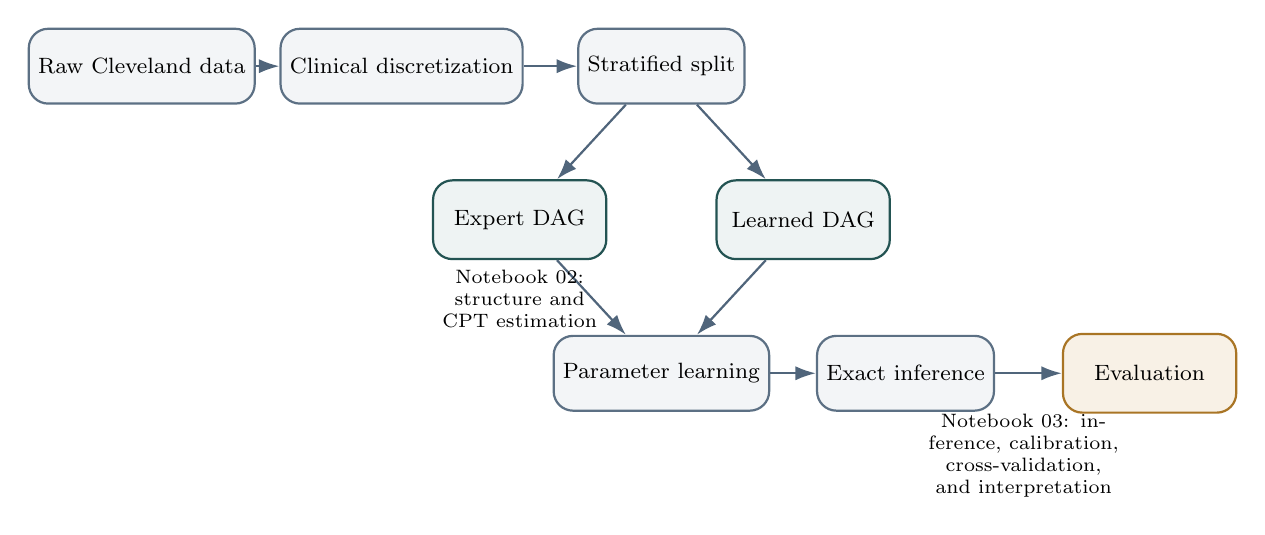
\begin{tikzpicture}[x=1cm,y=1cm]
  \node[flowbox] (raw) at (0.0,0.0) {Raw Cleveland data};
  \node[flowbox] (disc) at (3.3,0.0) {Clinical discretization};
  \node[flowbox] (split) at (6.6,0.0) {Stratified split};

  \node[modelbox] (expert) at (4.8,-1.95) {Expert DAG};
  \node[modelbox] (learned) at (8.4,-1.95) {Learned DAG};

  \node[flowbox] (fit) at (6.6,-3.9) {Parameter learning};
  \node[flowbox] (infer) at (9.7,-3.9) {Exact inference};
  \node[evalbox] (eval) at (12.8,-3.9) {Evaluation};

  \draw[dataarrow] (raw) -- (disc);
  \draw[dataarrow] (disc) -- (split);
  \draw[dataarrow] (split) -- (expert);
  \draw[dataarrow] (split) -- (learned);
  \draw[dataarrow] (expert) -- (fit);
  \draw[dataarrow] (learned) -- (fit);
  \draw[dataarrow] (fit) -- (infer);
  \draw[dataarrow] (infer) -- (eval);

  \node[font=\scriptsize, text width=2.8cm, align=center] at (4.8,-2.95) {Notebook 02: structure and CPT estimation};
  \node[font=\scriptsize, text width=3.0cm, align=center] at (11.2,-4.95) {Notebook 03: inference, calibration, cross-validation, and interpretation};
\end{tikzpicture}
\end{center}
\newpage

% Figure 2: Cohort bars
\begin{center}
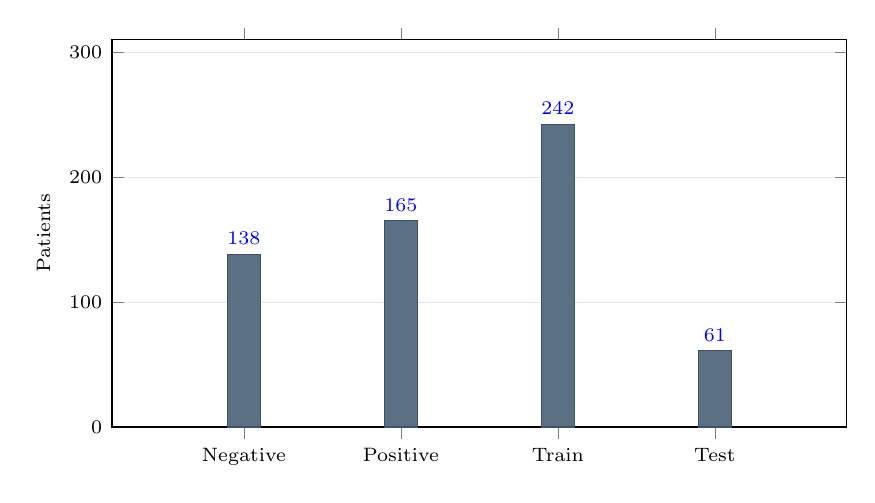
\begin{tikzpicture}
\begin{axis}[
    width=0.9\textwidth,
    height=6.5cm,
    ybar,
    bar width=12pt,
    ymin=0,
    ymax=310,
    enlarge x limits=0.28,
    symbolic x coords={Negative,Positive,Train,Test},
    xtick=data,
    ylabel={Patients},
    ymajorgrids=true,
    grid style={gray!20},
    tick label style={font=\scriptsize},
    label style={font=\scriptsize},
    nodes near coords,
    every node near coord/.append style={font=\scriptsize}
]
\addplot+[fill=navy!70, draw=navy!85] coordinates {
  (Negative,138)
  (Positive,165)
  (Train,242)
  (Test,61)
};
\end{axis}
\end{tikzpicture}
\end{center}
\newpage

% Figure 3: Structure composite
\begin{center}
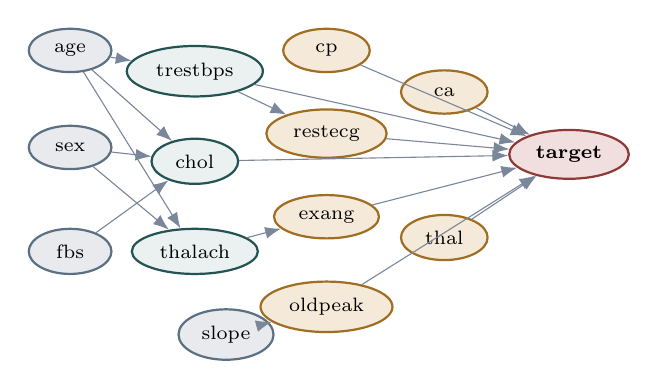
\begin{tikzpicture}[scale=0.88]
  \node[dagroot]   (age)      at (-4.4,  1.8) {age};
  \node[dagroot]   (sex)      at (-4.4,  0.4) {sex};
  \node[dagroot]   (fbs)      at (-4.4, -1.1) {fbs};
  \node[dagroot]   (slope)    at (-2.15, -2.3) {slope};

  \node[dagnode]   (trestbps) at (-2.6,  1.5) {trestbps};
  \node[dagnode]   (chol)     at (-2.6,  0.2) {chol};
  \node[dagnode]   (thalach)  at (-2.6, -1.1) {thalach};
  \node[dagparent] (cp)       at (-0.7,  1.8) {cp};
  \node[dagparent] (restecg)  at (-0.7,  0.6) {restecg};
  \node[dagparent] (exang)    at (-0.7, -0.6) {exang};
  \node[dagparent] (oldpeak)  at (-0.7, -1.9) {oldpeak};
  \node[dagparent] (ca)       at ( 1.0,  1.2) {ca};
  \node[dagparent] (thal)     at ( 1.0, -0.9) {thal};
  \node[dagtarget] (target)   at ( 2.8,  0.3) {target};

  \draw[dagar] (age) -- (trestbps);
  \draw[dagar] (age) -- (chol);
  \draw[dagar] (age) -- (thalach);
  \draw[dagar] (sex) -- (chol);
  \draw[dagar] (sex) -- (thalach);
  \draw[dagar] (fbs) -- (chol);
  \draw[dagar] (trestbps) -- (restecg);
  \draw[dagar] (thalach) -- (exang);
  \draw[dagar] (slope) -- (oldpeak);
  \draw[dagar] (cp) -- (target);
  \draw[dagar] (chol) -- (target);
  \draw[dagar] (trestbps) -- (target);
  \draw[dagar] (restecg) -- (target);
  \draw[dagar] (exang) -- (target);
  \draw[dagar] (oldpeak) -- (target);
  \draw[dagar] (ca) -- (target);
  \draw[dagar] (thal) -- (target);
\end{tikzpicture}

\vspace{1cm}

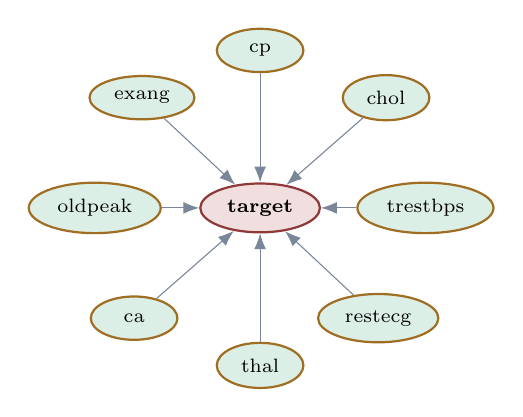
\begin{tikzpicture}[scale=1.0]
  \node[dagtarget] (t) at (0,0) {target};
  \node[dagparent, fill=blanket] (cpb)       at ( 0.0,  2.0) {cp};
  \node[dagparent, fill=blanket] (cholb)     at ( 1.6,  1.4) {chol};
  \node[dagparent, fill=blanket] (trestb)    at ( 2.1,  0.0) {trestbps};
  \node[dagparent, fill=blanket] (restecgb)  at ( 1.5, -1.4) {restecg};
  \node[dagparent, fill=blanket] (thalb)     at ( 0.0, -2.0) {thal};
  \node[dagparent, fill=blanket] (cab)       at (-1.6, -1.4) {ca};
  \node[dagparent, fill=blanket] (oldpeakb)  at (-2.1,  0.0) {oldpeak};
  \node[dagparent, fill=blanket] (exangb)    at (-1.5,  1.4) {exang};

  \foreach \x in {cpb,cholb,trestb,restecgb,thalb,cab,oldpeakb,exangb}
    \draw[dagar] (\x) -- (t);
\end{tikzpicture}
\end{center}
\newpage

% Figure 4: Scorecard
\begin{center}
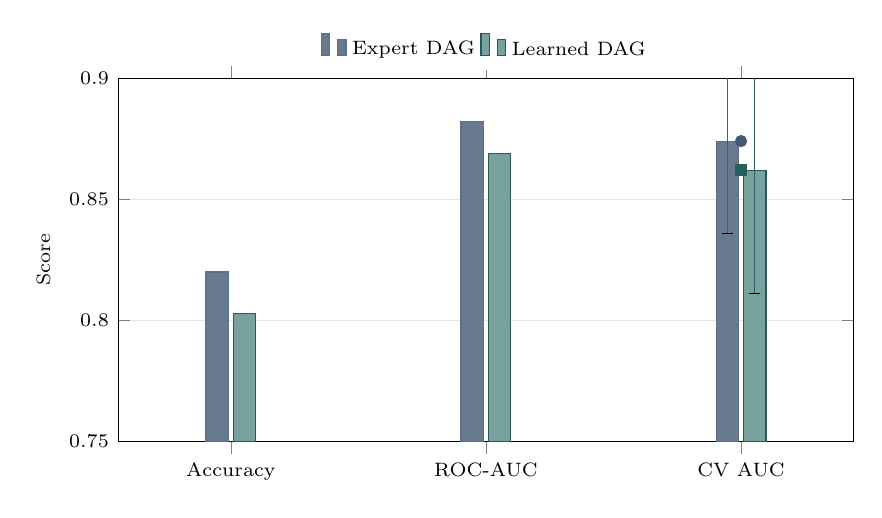
\begin{tikzpicture}
\begin{axis}[
    width=0.9\textwidth,
    height=6.2cm,
    ybar,
    bar width=8pt,
    ymin=0.75,
    ymax=0.90,
    enlarge x limits=0.22,
    symbolic x coords={Accuracy,ROC-AUC,CV AUC},
    xtick=data,
    ylabel={Score},
    ymajorgrids=true,
    grid style={gray!20},
    legend style={at={(0.5,1.02)},anchor=south,legend columns=2,draw=none,font=\scriptsize},
    tick label style={font=\scriptsize},
    label style={font=\scriptsize}
]
\addplot+[fill=navy!65, draw=navy!70] coordinates {
  (Accuracy,0.820)
  (ROC-AUC,0.882)
  (CV AUC,0.874)
};
\addplot+[fill=teal!65, draw=teal!80!black] coordinates {
  (Accuracy,0.803)
  (ROC-AUC,0.869)
  (CV AUC,0.862)
};
\legend{Expert DAG, Learned DAG}

\addplot[
  only marks,
  mark=*,
  mark options={fill=navy!80,draw=navy!80},
  draw=navy!80,
  error bars/y dir=both,
  error bars/y explicit,
  error bars/error bar style={draw=navy!80}
] coordinates {(CV AUC,0.874) +- (0,0.038)};

\addplot[
  only marks,
  mark=square*,
  mark options={fill=teal!85!black,draw=teal!85!black},
  draw=teal!85!black,
  error bars/y dir=both,
  error bars/y explicit,
  error bars/error bar style={draw=teal!85!black}
] coordinates {(CV AUC,0.862) +- (0,0.051)};
\end{axis}
\end{tikzpicture}
\end{center}
\newpage

% Figure 5: Brier bars
\begin{center}
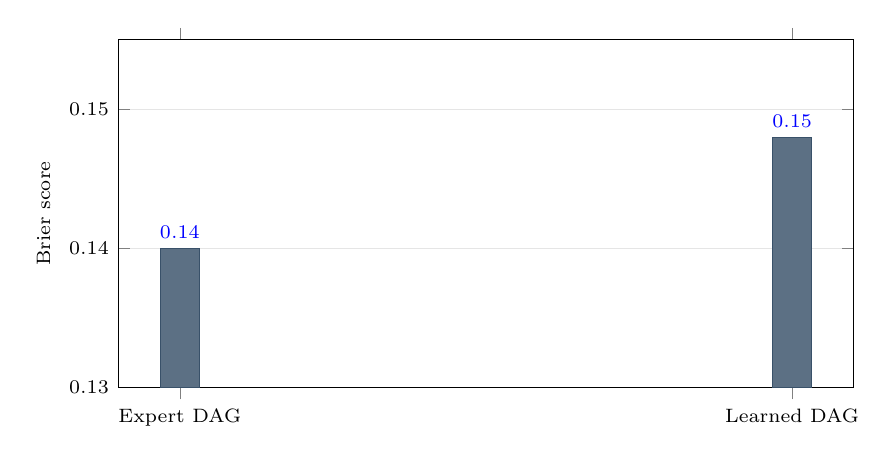
\begin{tikzpicture}
\begin{axis}[
    width=0.9\textwidth,
    height=6.0cm,
    ybar,
    bar width=14pt,
    ymin=0.13,
    ymax=0.155,
    symbolic x coords={Expert DAG,Learned DAG},
    xtick=data,
    ylabel={Brier score},
    ymajorgrids=true,
    grid style={gray!20},
    tick label style={font=\scriptsize},
    label style={font=\scriptsize},
    nodes near coords,
    every node near coord/.append style={font=\scriptsize}
]
\addplot+[fill=navy!70, draw=navy!85] coordinates {
  (Expert DAG,0.140)
  (Learned DAG,0.148)
};
\end{axis}
\end{tikzpicture}
\end{center}

\end{document}
